\section{Experiment Setup and Testing Methodology}
\label{sec:methodology}

The objective of this experiment is to evaluate the performance of these multi-agent AI systems and observe its accuracy in solving a multitude of mathematical problems. These results will be compared to the performance of a single AI agent in order to contextualize these results and show the difference in accuracy, efficiency, and scalability of these different approaches.

This hierarchical debate system is important because LLMs are known to occasionally produce incorrect and inconsistent responses. The goal of this experimentation is to show whether the hierarchical debate system and iterative refinement would lead to more accurate and reliable outputs. More specifically, this experiment aims to evaluate whether hierarchy depth further increases the accuracy at which the sample questions are answered.

\subsection{Test 1: Smaller Hierarchy}
The first test is designed to test a zero-shot AI agent against a multi-agent hierarchical system, following the "ABB" structure. This structure consists of one primary subnode, with two subordinate agents in the subnode. There are also support agents, those being the Prompt Generator, Counter, Checker, and Chat Manager.

\begin{figure}[h]
    \centering
    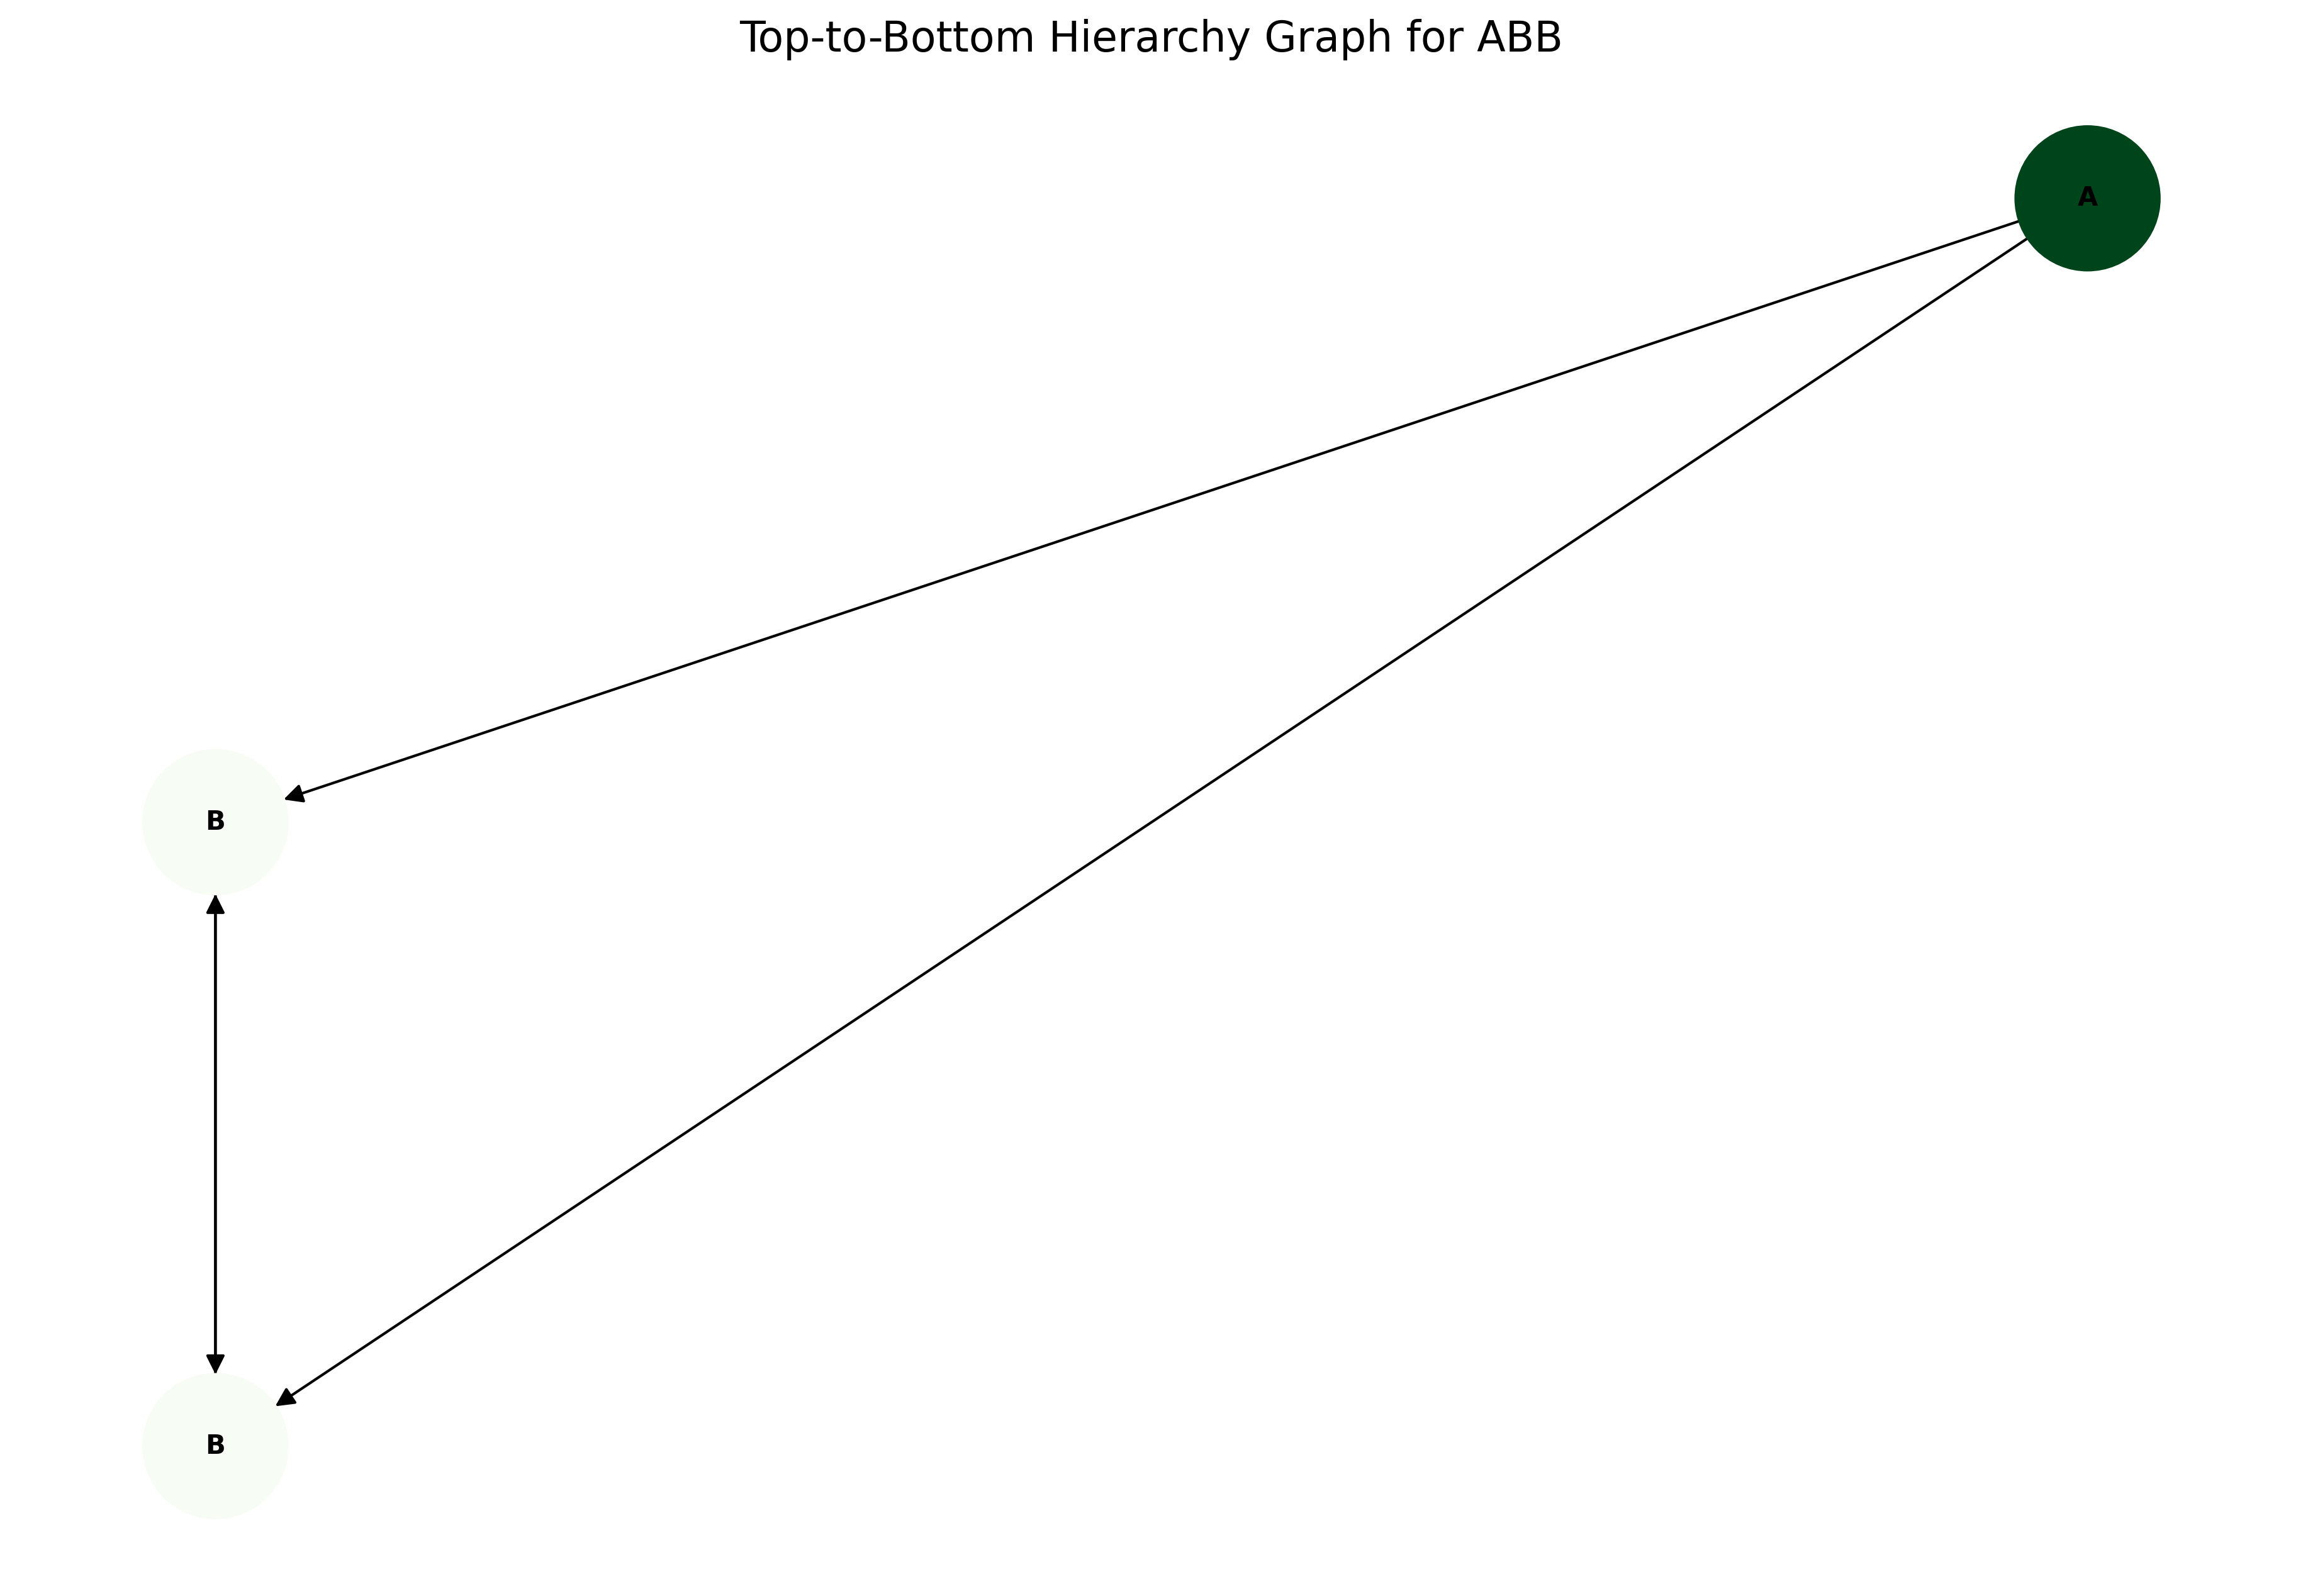
\includegraphics[width=0.8\textwidth]{img/section_methodology/ABB.png}
    \caption{A Visualization of the Smaller "ABB" Hierarchy}
    \label{fig:smaller}
\end{figure}

Both the zero-shot AI agent and the "ABB" multi-agent hierarchy will be tasked with solving a set of 1000 questions, and then checked against an answer key. This experiment will establish a baseline comparison between the zero-shot agent and the simple-hierarchy multi-agent system. This will establish the effect of a small amount of collaboration between agents on solving problems. 

\subsection{Test 2: Large Hierarchy}
Similarly to the first test, this second test will evaluate the performance of a zero-shot AI agent compared to a hierarchical system. However, this will be with the more complex hierarchical structure "ABCCBCCC". This structure has one Gen 0 subnode, two Gen 1 subnodes, seven subordinate agents, and then the same support agents. 

\begin{figure}[h]
    \centering
    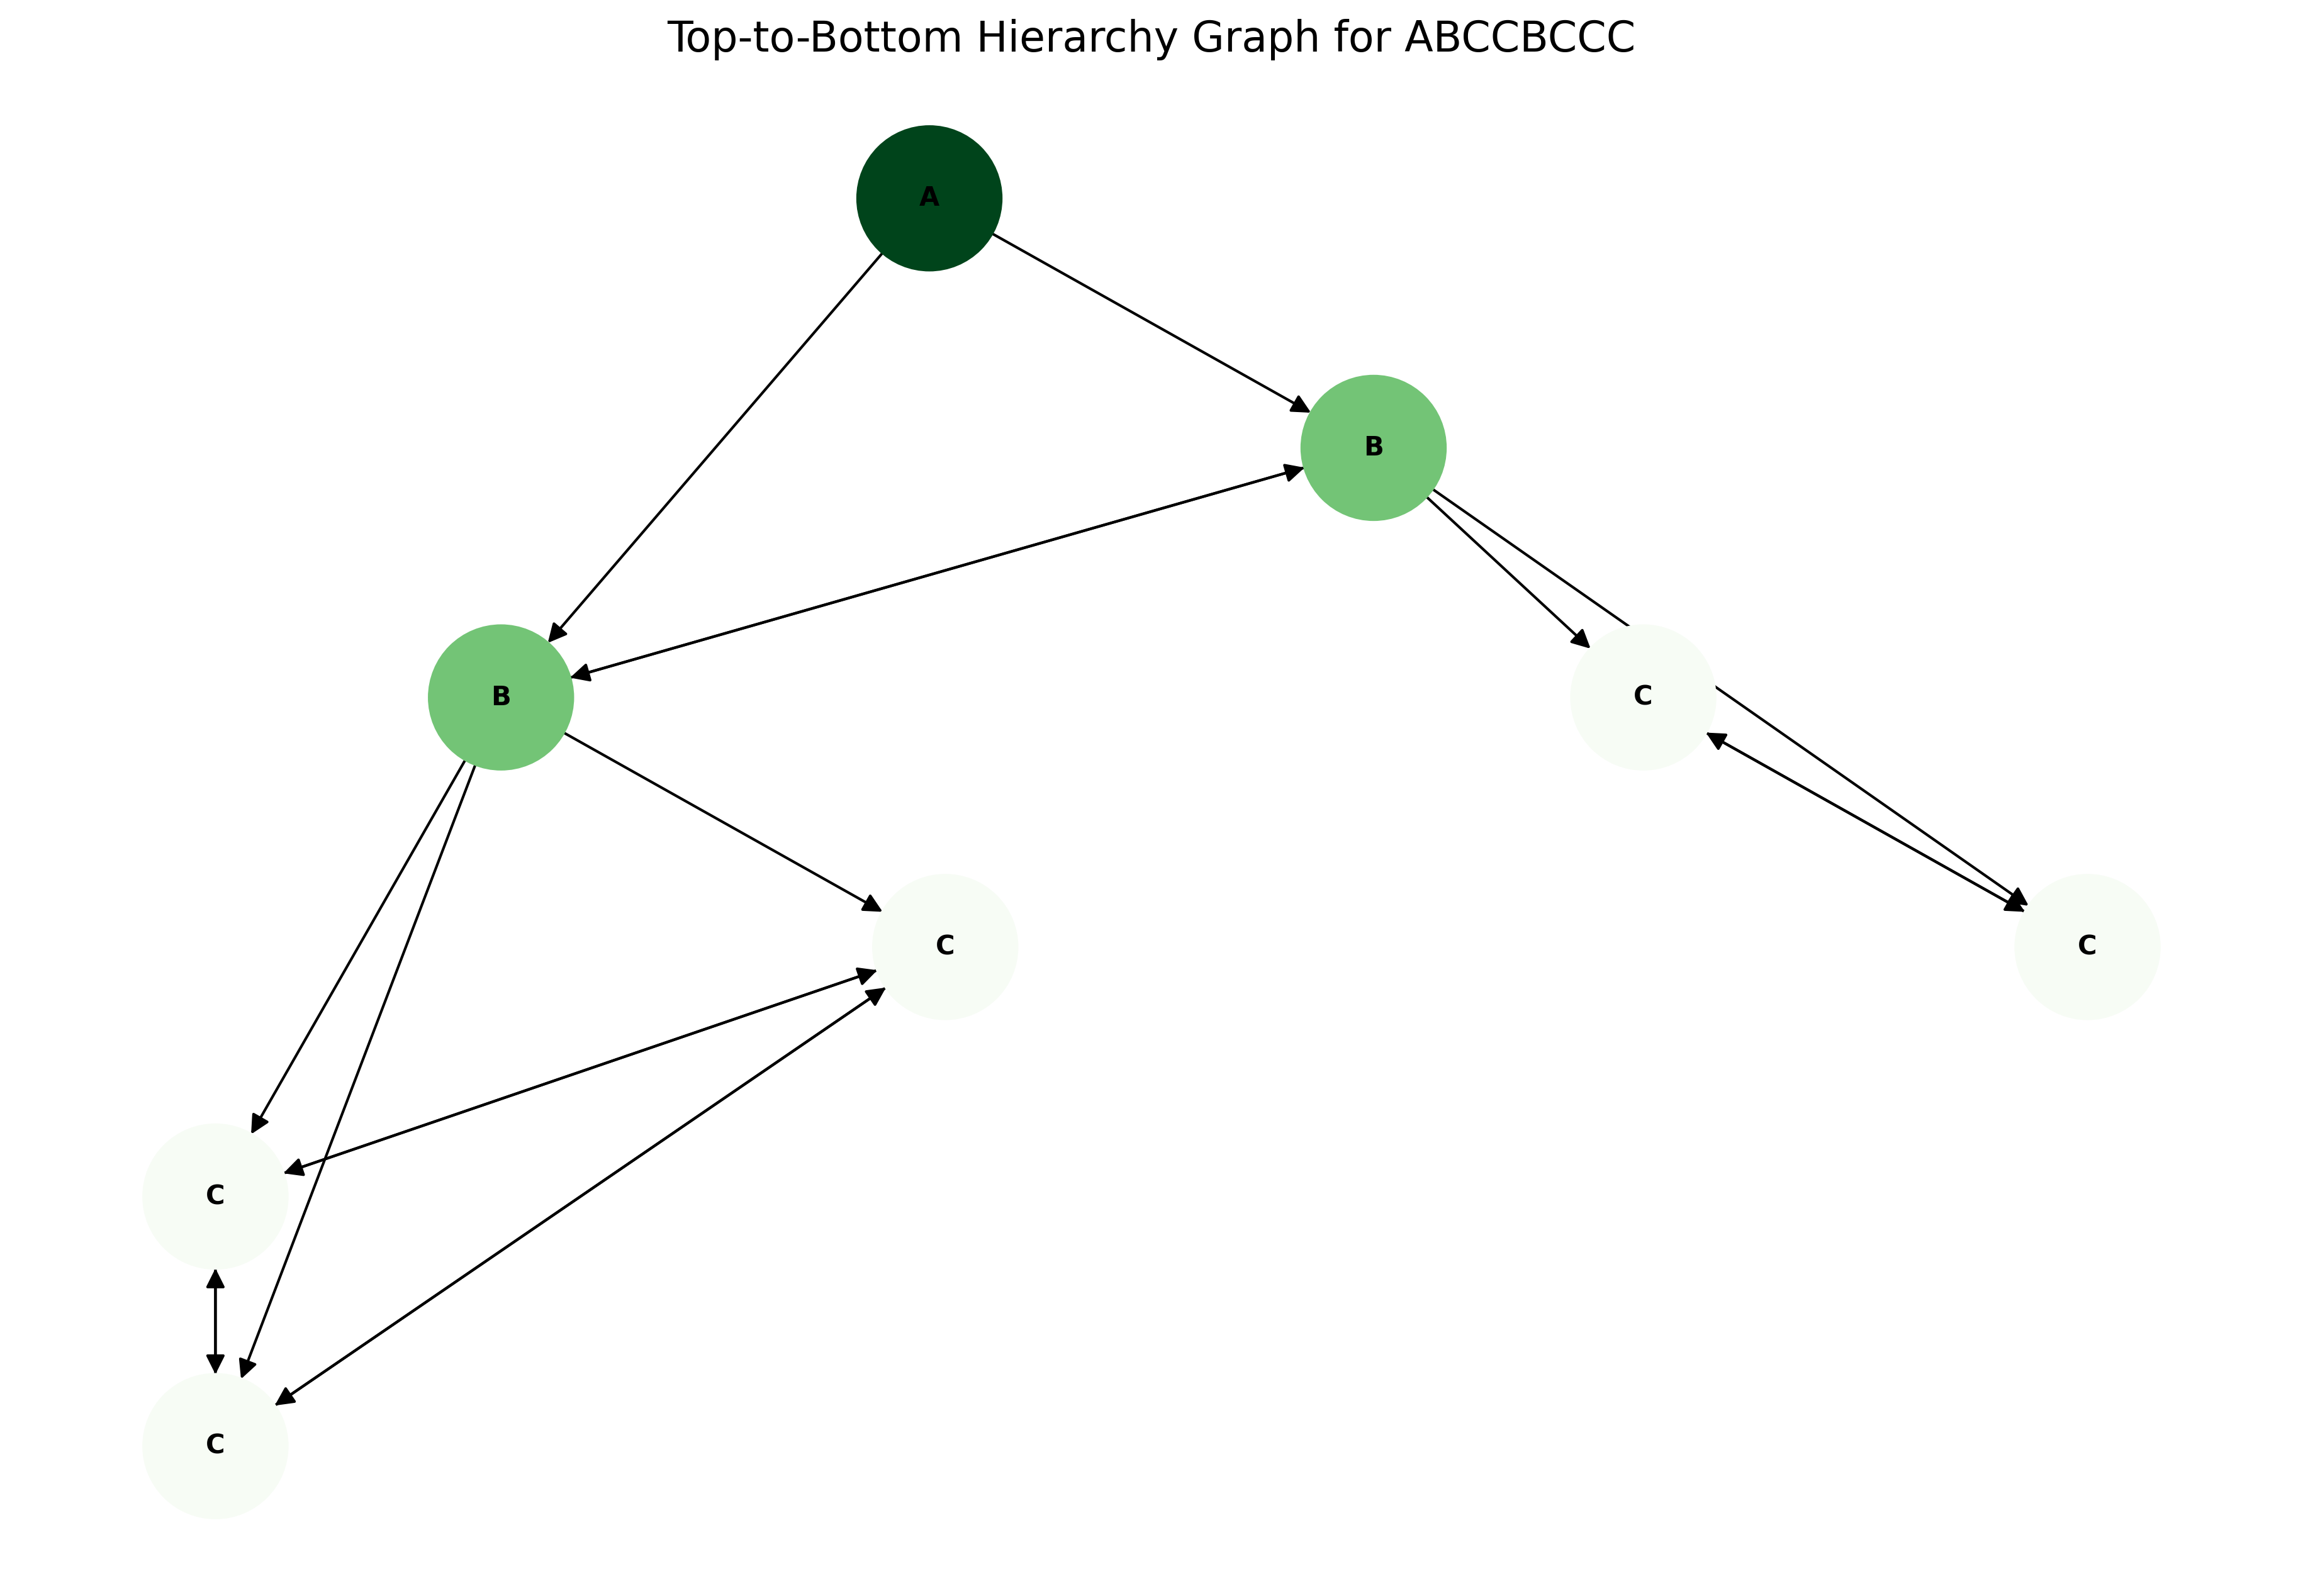
\includegraphics[width=0.8\textwidth]{img/section_methodology/ABCCBCCC.png}
    \caption{A Visualization of the Large "ABCCBCC" Hierarchy}
    \label{fig:large}
\end{figure}

In this test, both the zero-shot AI agent and the "ABCCBCCC" structure will be tasked with solving 200 questions and then checked against the answer key. While this test contains fewer questions than the first one, this is to compensate for the additional computing time due to the complex structure in this version. This test will evaluate whether the deeper hierarchies lead to better accuracy compared to the simpler hierarchies, and how that compares to the added computational intensity.

Through testing with both a simple hierarchy and a complex hierarchy, we will evaluate the practical difference in output between having a multi-agent debate structure, the complexity of the structure, and how the scalability affects the computational intensity.

\subsection{Testing Procedure}
The process the different AI structures followed in answering questions and providing results were done systematically, ensuring structure, consistency, and reproducibility. Each of these tests consists of question selection, execution by the agent, evaluation, and then storing the results.

\subsubsection{Question Selection}
The first part of the experiment is choosing a question for both structures to answer. These questions were sourced from a dataset containing mathematical problems, and also had the correct numerical answer for each question. For Test 1, we randomly selected 1000 questions, and for Test 2, we randomly selected 200 questions. Test 2 contained less questions due to the time complexity of the "ABCCBCCC" structure.

\subsubsection{Agent Execution}
Each question was processed in parallel by both the zero-shot agent and the multi-agent debate system. While the zero-shot agent was only prompted once to generate a response, the multi-agent model processed it in its hierarchical structure. The Prompt Generator Agent structured the problem, the Subordinate Agents independently tried to solve the problem, and the Checker Agent determined whether various answers converged. Until this convergence was achieved, the multi-agent debate continued across multiple rounds. For computational purposes and preventing an infinite loop, the maximum number of debate rounds was capped to 21.

\subsubsection{Evaluation}
Each answer by the AI systems were compared against the true answer provided by the dataset using an automated function. Since the problems were mathematical problems, the responses were parsed to extract only the numerical values, and this was compared against the benchmark answer. If the extracted numerical value was accurate within a tolerance of 1e-6, then it was marked as correct. Otherwise, it was marked incorrect.
The metrics that were tracked are: correct/incorrect responses, response times for both the single agent and the multi-agent system, and the round count for the multi-agent system. These are all necessary metrics to track the accuracy of both systems as well as the computational difference.

\subsubsection{Data Storage}
For structure and reproducibility, the test data was stored in a clear hierarchical format, ensuring easy accessibility to any necessary test data. Each test is stored in its own folder, containing: hierarchy visualization, summary of performance metrics, and stored conversation logs in another folder.

\subsection{Expected Outcomes}
We expect to see trade-offs between the different systems given their unique structures, across accuracy, execution time, and scalability. Accuracy can be expected to increase with the complexity of the system and the number of agents, so we would expect the "ABCCBCCC" multi-agent model to be the most accurate, with the simpler "ABB" structure being second and the zero-shot model being the lowest. As for execution time, the reverse would be true, with the simplest zero-shot model being the fastest and the large hierarchical model being the slowest. As for scalability, we would expect there to be diminishing returns in accuracy compared to computation meaning that the difference in performance would degrade with the depth of the hierarchy.